\subsection{Testing}
\subsubsection{Analisi Statica - CodMR}

Lorem ipsum dolor sit amet, consectetur adipiscing elit. Nam sit amet arcu quis purus porttitor ullamcorper. Nullam eget tincidunt ligula. Nulla facilisi. Phasellus vehicula, quam ac auctor pharetra, augue justo gravida velit, at tristique urna ligula a felis. Vestibulum fermentum vehicula turpis, ut sagittis dolor pharetra in. Suspendisse potenti. Duis non felis eget erat volutpat consequat. Curabitur a enim nec eros fermentum interdum a vel dui. 

Vivamus scelerisque varius massa, eget tristique risus pellentesque ac. Integer vitae dolor id quam suscipit scelerisque non in eros. Maecenas id felis eget ligula vestibulum condimentum. Ut in tellus eget metus suscipit gravida. In faucibus arcu eget libero laoreet, non eleifend tortor maximus. Aenean vitae purus et velit eleifend venenatis. Quisque nec metus a arcu tincidunt ultricies. Morbi sit amet felis auctor, consequat erat id, ultricies sapien. 

Curabitur tristique neque at mauris auctor, sit amet vehicula arcu tincidunt. Integer ac bibendum lectus. Phasellus eu orci at lorem scelerisque tempor sed vel leo. Nullam elementum vel tortor a tempus. Aliquam erat volutpat. Pellentesque in consectetur justo. Donec id leo neque. Duis scelerisque pharetr


\subsubsection{Analisi Dinamica - JUnit}
Lorem ipsum dolor sit amet, consectetur adipiscing elit. Nam sit amet arcu quis purus porttitor ullamcorper. Nullam eget tincidunt ligula. Nulla facilisi. Phasellus vehicula, quam ac auctor pharetra, augue justo gravida velit, at tristique urna ligula a felis. Vestibulum fermentum vehicula turpis, ut sagittis dolor pharetra in. Suspendisse potenti. Duis non felis eget erat volutpat consequat. Curabitur a enim nec eros fermentum interdum a vel dui. 

Vivamus scelerisque varius massa, eget tristique risus pellentesque ac. Integer vitae dolor id quam suscipit scelerisque non in eros. Maecenas id felis eget ligula vestibulum condimentum. Ut in tellus eget metus suscipit gravida. In faucibus arcu eget libero laoreet, non eleifend tortor maximus. Aenean vitae purus et velit eleifend venenatis. Quisque nec metus a arcu tincidunt ultricies. Morbi sit amet felis auctor, consequat erat id, ultricies sapien. 

Curabitur tristique neque at mauris auctor, sit amet vehicula arcu tincidunt. Integer ac bibendum lectus. Phasellus eu orci at lorem scelerisque tempor sed vel leo. Nullam elementum vel tortor a tempus. Aliquam erat volutpat. Pellentesque in consectetur justo. Donec id leo neque. Duis scelerisque pharetr

\subsubsection{API Esposte}

Questa sezione documenta le API principali del sistema \textbf{Spendly}, includendo autenticazione, gestione dei gruppi e visualizzazione. Ogni test verrà mostrato con un' \texttt{immagine dei risultati}.

\paragraph{Registrazione Utente}
\begin{itemize}
    \item \textbf{Endpoint:} \texttt{POST /account/register}
    \item \textbf{Descrizione:} Consente a un nuovo utente di registrarsi al sistema.
    \item \textbf{Parametri:}
    \begin{itemize}
        \item \texttt{nome} (string) - Nome utente.
        \item \texttt{cognome} (string) - Nome utente.
        \item \texttt{username} (string) - Username utente(non accetta duplicati).
        \item \texttt{email} (string) - Email dell'utente(non accetta duplicati).
        \item \texttt{telefono} (string) - Telefono utente.
        \item \texttt{indirizzo} (string) - Indirizzo utente.
        \item \texttt{password} (string) - Password scelta dall'utente.
    \end{itemize}
    \item \textbf{Risultato:}
\end{itemize}
\begin{figure}[H]
    \centering
    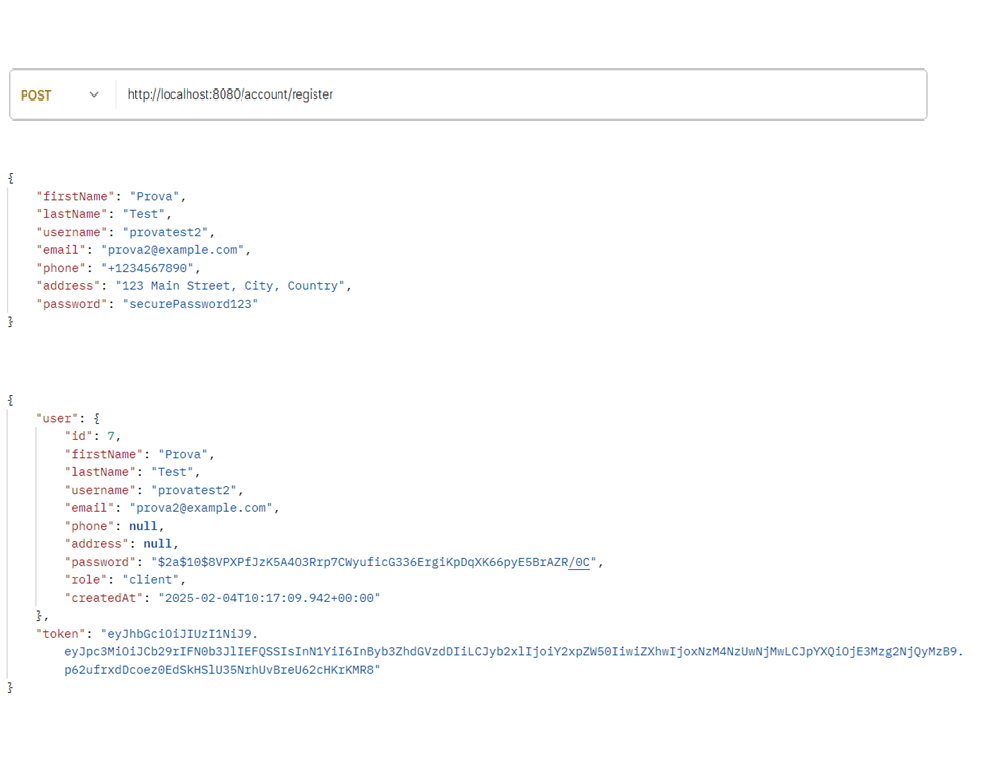
\includegraphics[width=0.9\textwidth]{images/registerapi.png}
    \caption{Risultato API Registrazione}
    \label{fig:api_register}
\end{figure}

\paragraph{Login Utente}
\begin{itemize}
    \item \textbf{Endpoint:} \texttt{POST /account/login}
    \item \textbf{Descrizione:} Permette a un utente registrato di accedere al sistema.
    \item \textbf{Parametri:}
    \begin{itemize}
        \item \texttt{username} (string) - Username dell'utente.
        \item \texttt{password} (string) - Password dell'utente.
    \end{itemize}
    \item \textbf{Risultato:}  
\end{itemize}
\begin{figure}[H]
    \centering
    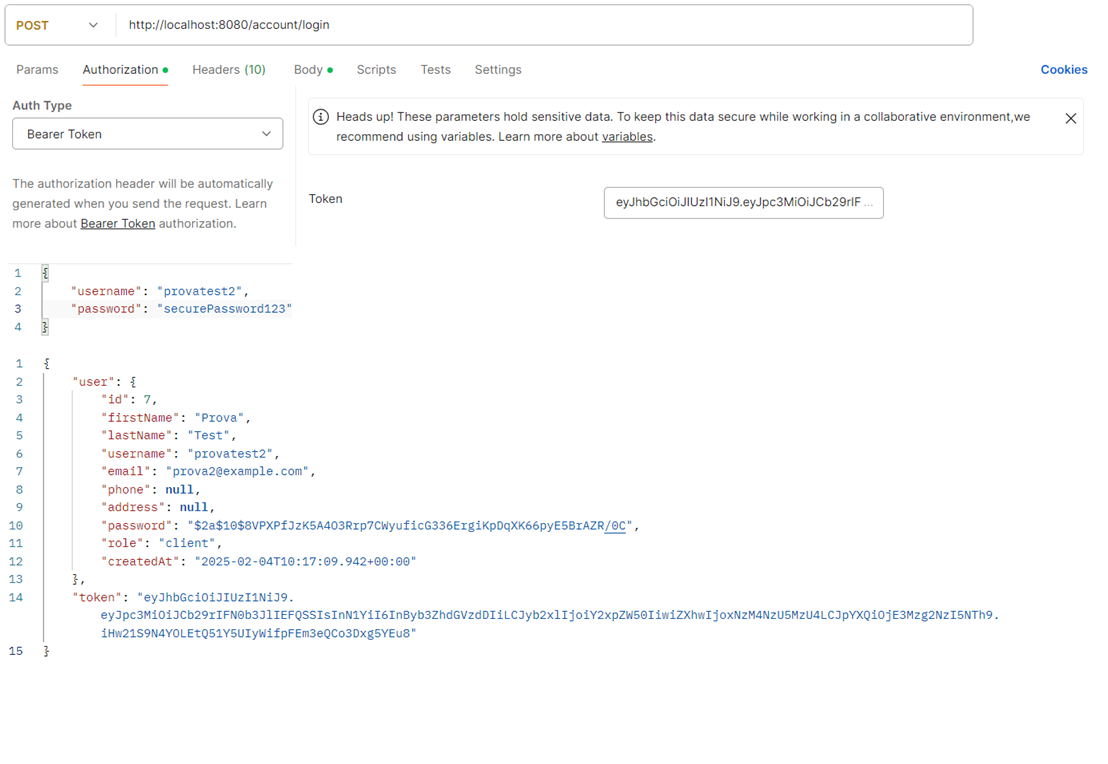
\includegraphics[width=0.9\textwidth]{images/loginapi.png}
    \caption{Risultato API Login}
    \label{fig:api_login}
\end{figure}

\paragraph{Creazione di un Gruppo}
\begin{itemize}
    \item \textbf{Endpoint:} \texttt{POST /api/groups}
    \item \textbf{Descrizione:} Permette la creazione di un nuovo gruppo da parte dell'utente.
    \item \textbf{Parametri:}
    \begin{itemize}
        \item \texttt{name} (string) - Nome del gruppo.
        \item \texttt{username} (string) - Username dell'utente che crea il gruppo.
    \end{itemize}
    \item \textbf{Risultato:}
\end{itemize}
\begin{figure}[H]
    \centering
    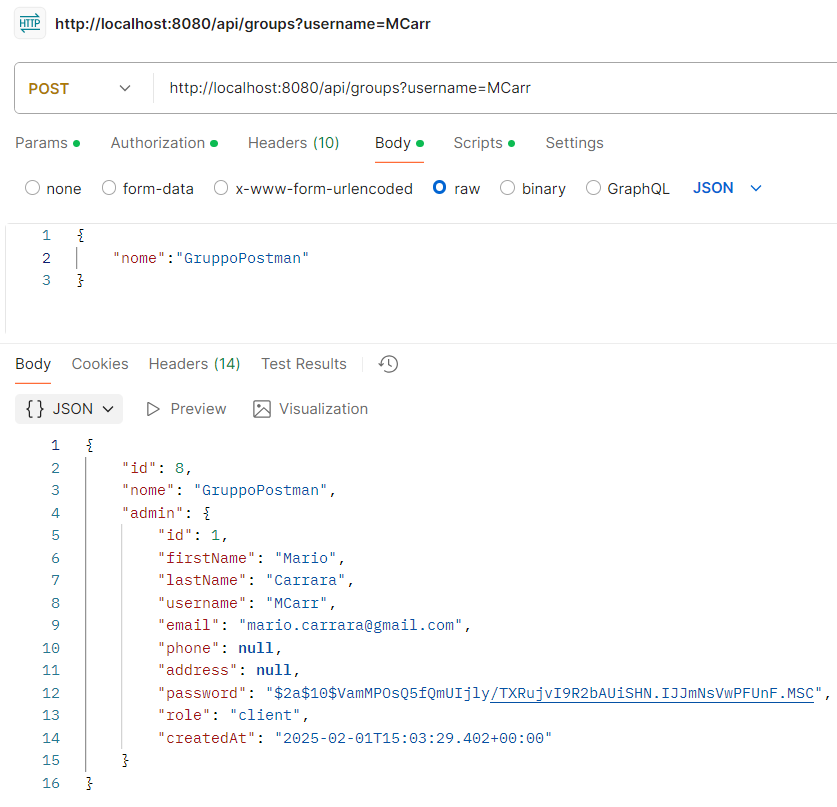
\includegraphics[width=0.8\textwidth]{images/CreateGroupAPI.png}
    \caption{Risultato API Creazione Gruppo}
    \label{fig:api_create_group}
\end{figure}

\paragraph{Inserimento di un utente in un gruppo}
\begin{itemize}
    \item \textbf{Endpoint:} \texttt{POST /api/groups/{group\_id}/members}
    \item \textbf{Descrizione:} Permette all'amministratore di inserire un utente in un gruppo.
    \item \textbf{Parametri:}
    \begin{itemize}
        \item \texttt{adminUsername} (string) - Username dell'admin del gruppo.
        \item \texttt{memberUsername} (string) - Username dell'utente da inserire.
    \end{itemize}
    \item \textbf{Risultato:}
\end{itemize}
\begin{figure}[H]
    \centering
    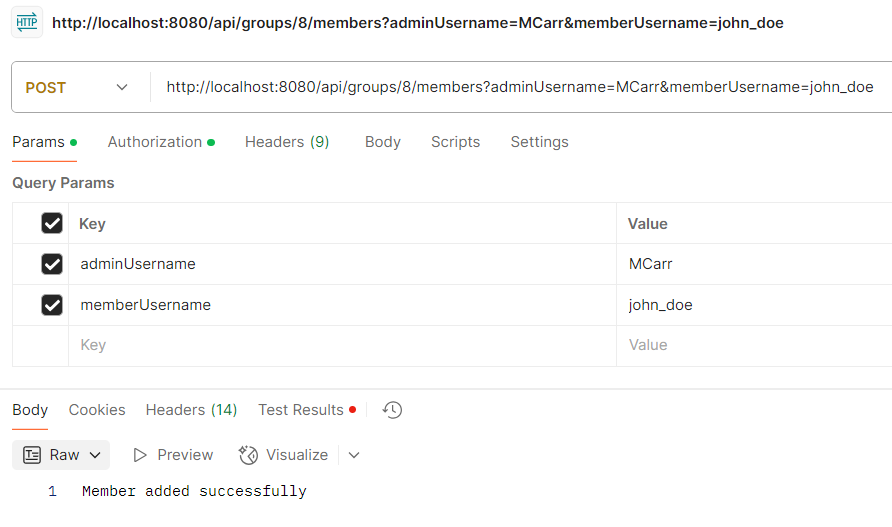
\includegraphics[width=0.8\textwidth]{images/AddMemberAPI.png}
    \caption{Risultato API Inserimento utente}
    \label{fig:api_add_member}
\end{figure}

\paragraph{Visualizzazione dei Gruppi}
\begin{itemize}
    \item \textbf{Endpoint:} \texttt{GET /api/groups}
    \item \textbf{Descrizione:} Restituisce la lista di tutti i gruppi a cui l'utente appartiene.
    \item \textbf{Parametri:}
    \begin{itemize}
        \item \texttt{username} (string) - Username dell'utente.
    \end{itemize}
    \item \textbf{Risultato:}
\end{itemize}
\begin{figure}[H]
    \centering
    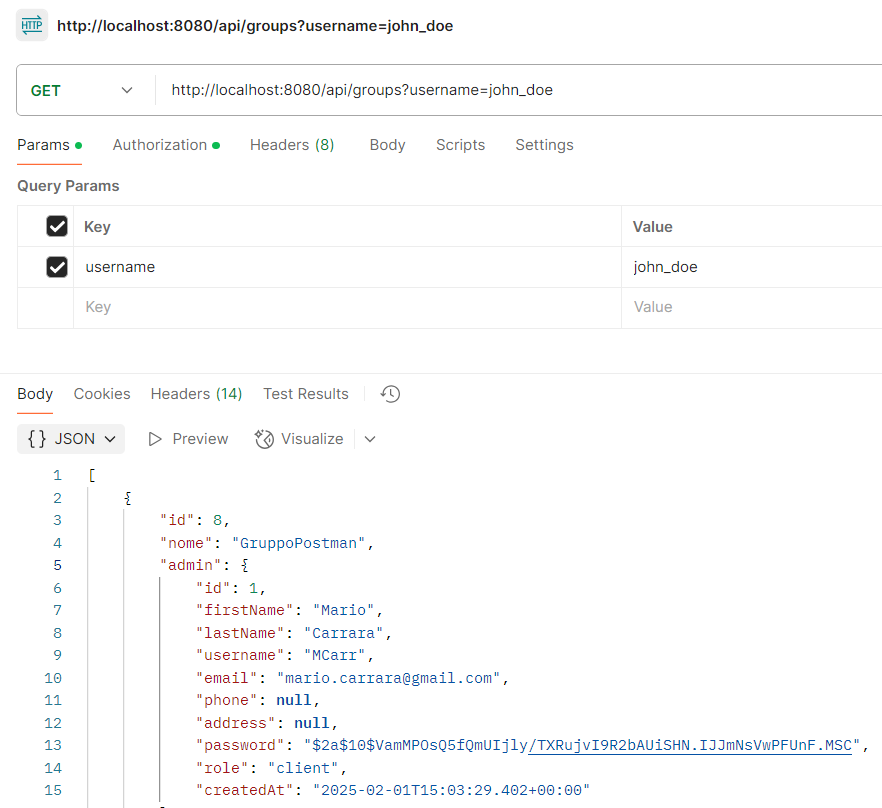
\includegraphics[width=0.8\textwidth]{images/GetAPI.png}
    \caption{Risultato API Visualizzazione Gruppi}
    \label{fig:api_view_groups}
\end{figure}

